\section{Shared memory parallelisation}
\label{section:shared-memory}

Three levels of multicore parallelisation:

- on the cell level
- within one 'cell' do all the particles in parallel
- within one particle-particle sweep, do all the triangles in parallel

We introduce three levels of shared memory parallelisation. On the highest level, we exploit the cell level decomposition and assign work within each cell to cores. Within the cell we assign work per particle pair  to an inner level of threads. Lastly within each particle pair the innermost level of parallelisation is utilised to exploit tessellation level parallelisation by the contact solver.

In the innermost level of parallesation we experimenting with three methods to resolve contact points in parallel. The first method is the brute force method where


\begin{figure}[!h]
\centering
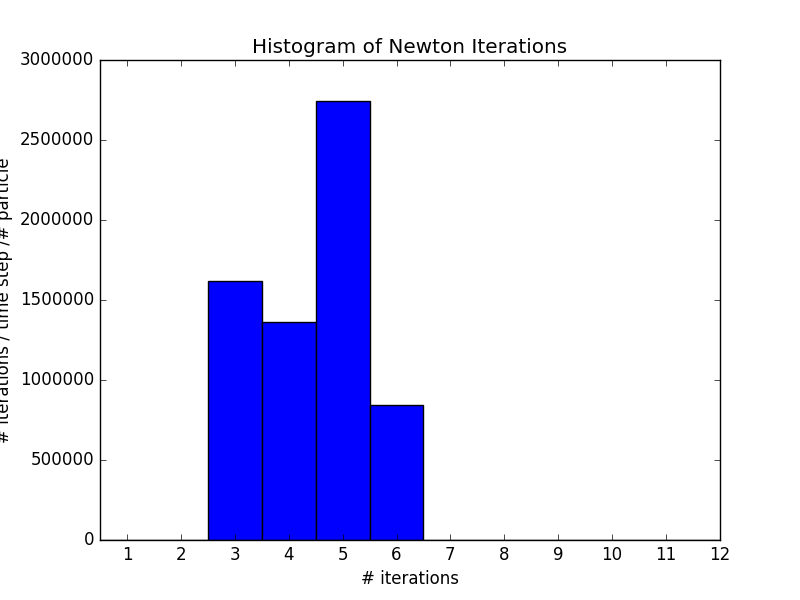
\includegraphics[width=1\textwidth]{experiments/random/newton_histogram} \protect\caption{\label{fig17}Newton solver histogram of number of iterations for convergence.}
\end{figure} 


\begin{figure}[!h]
\centering
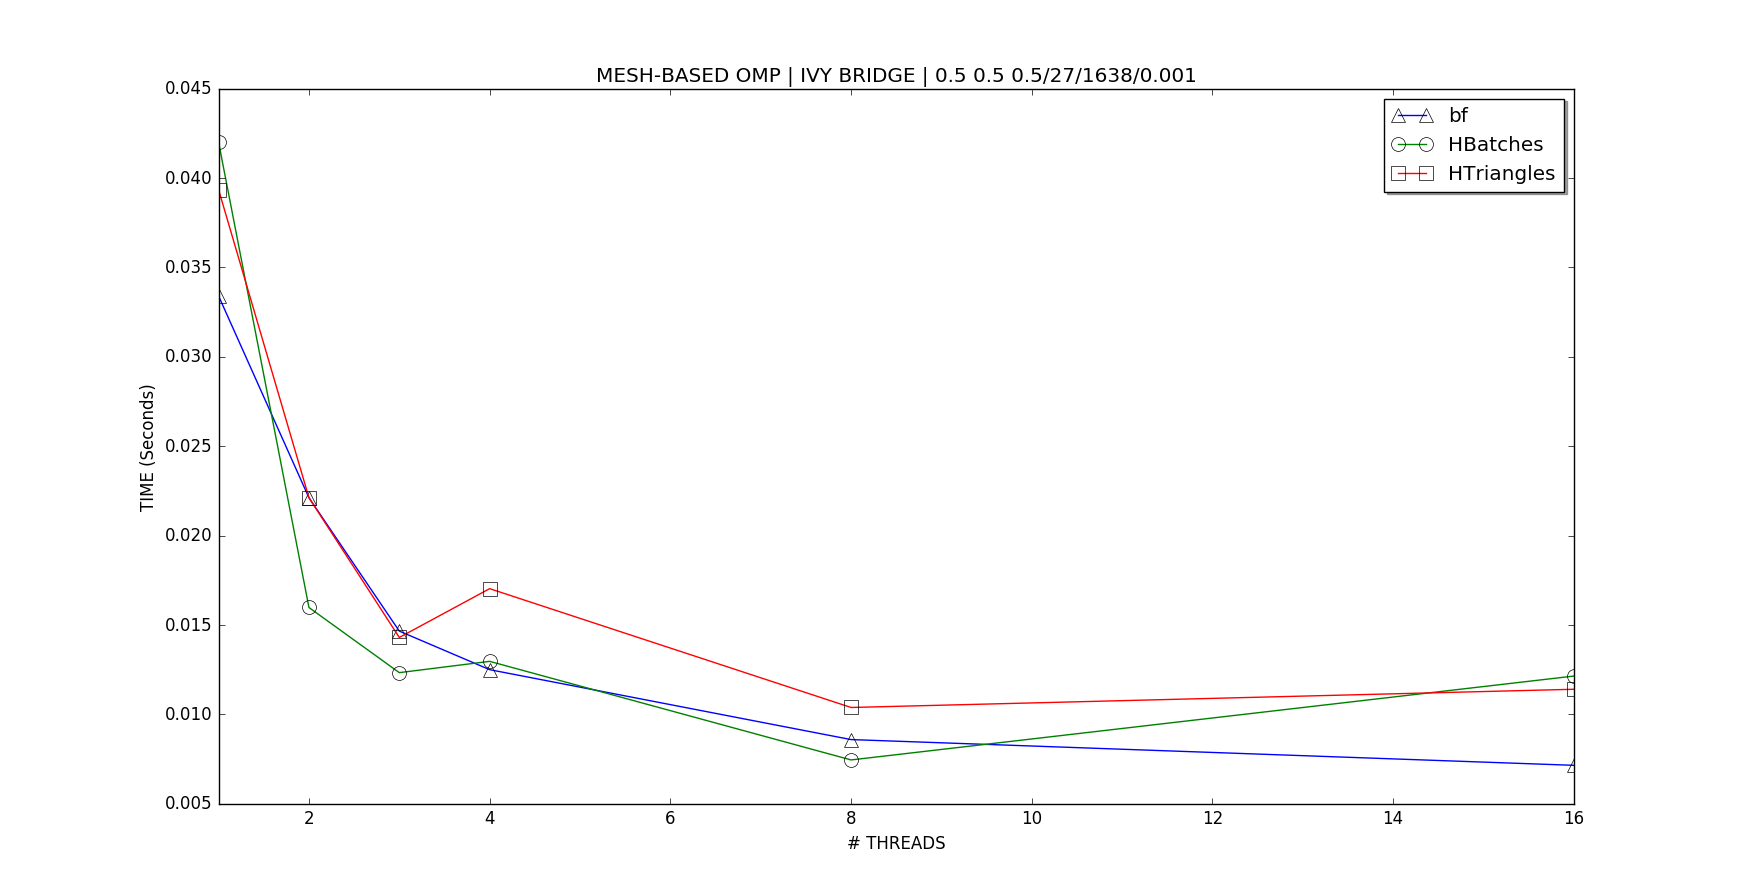
\includegraphics[width=1\textwidth]{experiments/random/triangle_based_x0} \protect\caption{\label{fig17} Triangle based shared memory parallelism using openMP.}
\end{figure} 


\begin{figure}[!h]
\centering
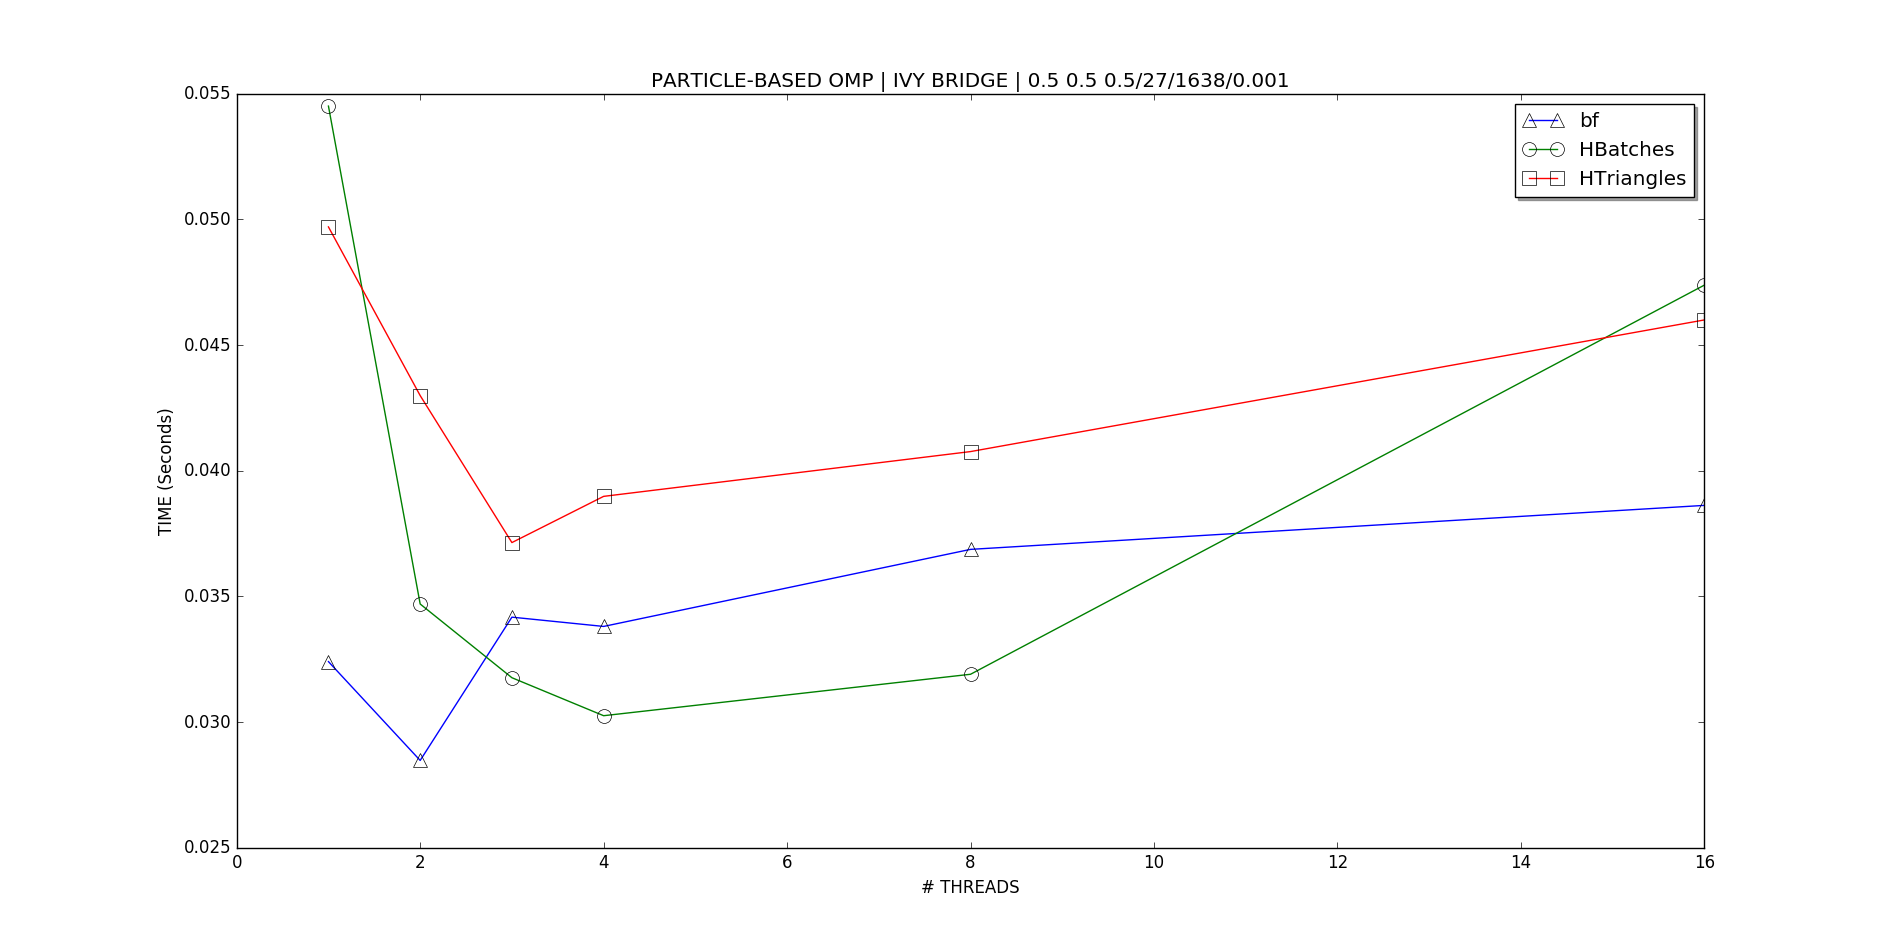
\includegraphics[width=1\textwidth]{experiments/random/particle_based_x0} \protect\caption{\label{fig17}Particle based shared memory parallelism using openMP.}
\end{figure} 


\begin{figure}[!h]
\centering
\includegraphics[width=1\textwidth]{experiments/random/particle_triangle_based_x0_based_x0} \protect\caption{\label{fig17}Particle and Triangle based nested shared memory parallelism using openMP.}
\end{figure} 

\begin{figure}[!h]
\centering
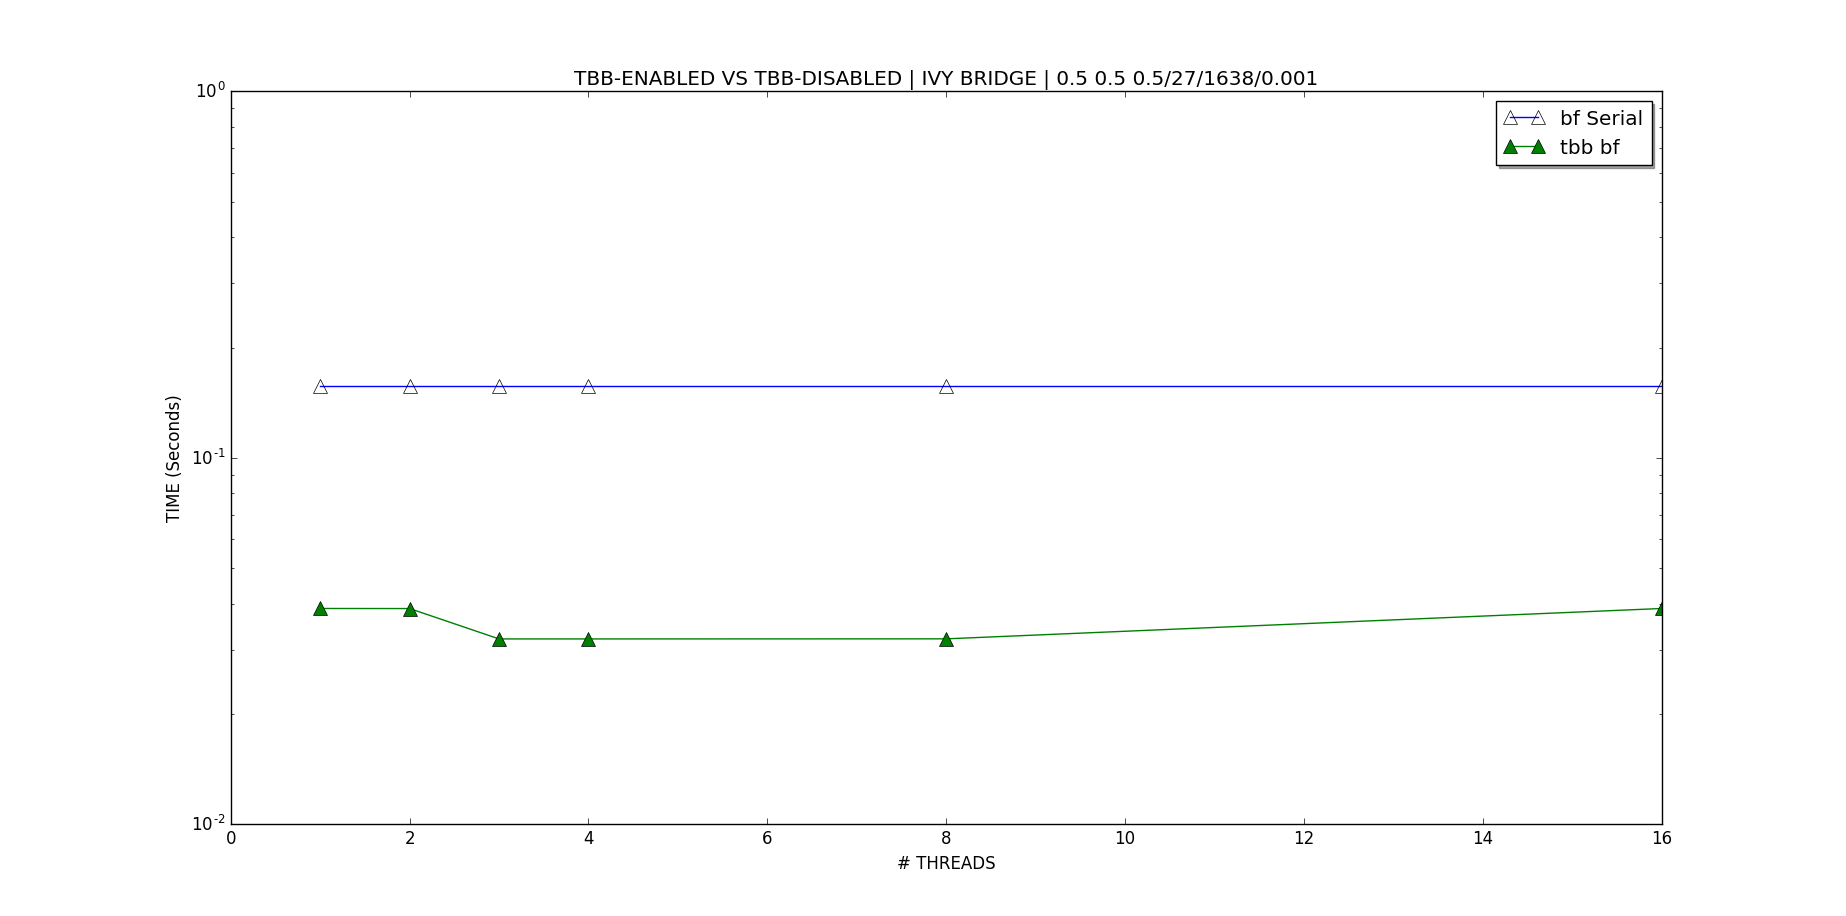
\includegraphics[width=1\textwidth]{experiments/random/tbb_vs_serial} \protect\caption{\label{fig17}Cell based parallelism compared to serial runs.}
\end{figure} 